This chapter describes learning models that are used to classify network traffic using deep learning.
The Deep Learning model used is the Convolution Neural Network (CNN), the Residual Network (ResNet), the Recurrent Neural Network (RNN), the Long Short-Term Memory LSTM) and the Convolution and Recurrent Neural Network (CNN + RNN).
The Deep Learning model was supported by Keras, and the ResNet and CNN + RNN models were generated using Keras' CNN and RNN models simultaneously.

CNN and ResNet models are commonly used for information extraction, sentence classification, face recognition, and image classification.
CNN extracts characteristics of data and grasps patterns of features.
RNN and LSTM are models specialized for repetitive and sequential data learning.
Therefore, the previous learning data is reflected in the current learning using the circulation structure.
It is generally used for the composition of speech, wave, and text.
Therefore, in the case of CNN and ResNet, it is used to classify using imaged packet unit data generated through preprocessing. RNN, LSTM, and CNN + RNN models are used to classify sequential data, so they are used to classify learning data in flow units that contain sequential information of network traffic.

\subsection{Convolution Neural Network Convolution Neural Network Architecture}
As shown in Fig. \ref{fig3}, the model architecture of CNN\cite{Krizhevsky:2012:ICD:2999134.2999257} is composed of the input layer, Convolution layer, and Pooling layer and Fully connected layer.
The input layer uses the payload and label of the packet converted into learning data. Packets are used as input data in the input layer in the form of $N \times N$ (N = 6, 8, 16, 32) like images.
Then, the feature of each packet data is convolved through the kernel of two Convolution layer, and output is generated through filter and activation process.
In the pooling layer, it is the process of reducing the size of the output through the convolution process.
It simply reduces the size of the data, cancels noise, and provides consistent features in fine detail.
Finally, the Fully connected layer extracts the prediction value according to the last 8 classes by activation.

\begin{figure}[t]
\centering
\setlength{\abovecaptionskip}{0pt}
\setlength{\belowcaptionskip}{0pt}
{
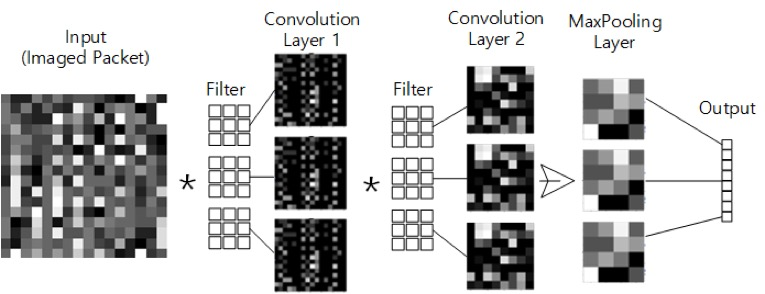
\includegraphics[width=3.6in]{fig3.jpg}
\caption{2-Layer CNN learning model architecture}
\label{fig3}
}
\end{figure}

\subsection{Residual Network Architecture}
Unlike traditional CNN, ResNet \cite{DBLP:journals:corr:HeZRS15} has a unique concept called shortcut connection.
A shortcut connection is added to the existing CNN model structure, and this shortcut is directly connected without any other parameters.
A shortcut connection is a type of adding a new type of network to an input value so that learning can be performed.
Therefore, the newly added network can achieve better performance while maintaining the performance of the existing learned network as much as possible.

\begin{figure*}[t]
\centering
\setlength{\abovecaptionskip}{0pt}
\setlength{\belowcaptionskip}{0pt}
{
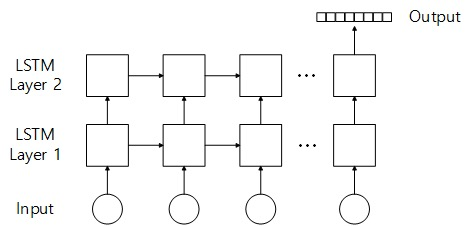
\includegraphics[scale=0.55]{fig4.jpg}
\caption{ResNet learning model architecture}
\label{fig4}
}
\end{figure*}

As shown in Fig. \ref{fig4}, when one packet of learning data enters the input, it passes through one convolution layer and one maxpooling layer.
The result through the maxpooling layer is then used as an input to one 3-convolution group.
Also, the maxpooling layer result is used as the input of the newly added shortcut network.
Thereafter, the output from one 3-convolution group and the output from the shortcut network are summed.
The result of the addition is passed through the Relu function again, and is used as the input of the second 3-convolution group and the shortcut network.
After three more iterations of the 3-convolution group process, the output after addition is sampled through the averagepooling layer and the result of the final classification comes out.

In terms of computation, there is nothing more than adding an operation.
Deep networks can be easily optimized through shortcut connections and can improve accuracy as depth increases.

\subsection{Recurrent Neural Network Architecture}
Recurrent Neural Network Architecture (RNN) \cite{J279188} is a network architecture that can accept inputs and outputs regardless of input data length and can be implemented variously and flexible as needed.
Therefore, the architecture of RNN used in this paper is composed of multi-layer as shown in Fig.\ref{fig5}.
In the RNN, the number of packets per flow (30, 60 and 100) is received at the input layer in order to learn flow unit data.
In the flow unit dataset, the first packet of one flow learning data is input to the first cell of the RNN layer.
The result of passing through the first RNN cell is used as an input at the same time when the next packet arrives at the input.
Therefore, the result of the first cell affects the operation of the second cell.
Also, the operation result of the first cell is used as the input of the second RNN layer.
At the same time, the operation result of the first cell of the second RNN layer is used as the input of the second cell.
The number of units to be set is then output to the number of applications learned in the output layer through the RNN cell.


\subsection{Long Short-Term Memory Architecture}
In addition to the existing RNN model, LSTM \cite{Hochreiter:1997:LSM:1246443.1246450} determines whether to keep the weight value by adding another feature layer called a cell state.
Through this, we solve the phenomenon that the weight value is not maintained as the distance between information and information of one input data in the existing RNN becomes longer, and the learning ability decreases.
LSTM is more persistent than existing RNN because it keeps updating the past data.
The cell state is responsible for adding or deleting information.
The architecture of the LSTM model is configured as shown in Fig.\ref{fig5}.

\begin{figure}[t]
\centering
\setlength{\abovecaptionskip}{0pt}
\setlength{\belowcaptionskip}{0pt}
{
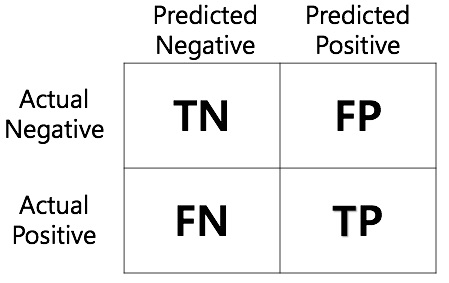
\includegraphics[width=3.6in]{fig5.jpg}
\caption{2-Layer RNN or LSTM learning model architecture}
\label{fig5}
}
\end{figure}

The advantage of LSTM is that each memory control is possible and the result can be controlled.
However, there is a possibility that the memory may be overwritten, and the operation speed is slower than that of the conventional RNN.
Therefore, it is composed of two layers different from existing RNN model.

\subsection{CNN and RNN Combination Network Model Architecture}
The learning model combining CNN and RNN is a combination of the convolution layer of CNN model and one LSTM layer.
As shown in Fig. \ref{fig6}, when the flow unit data set comes in as input, the image is compressed through the fiter of the convolution layer.
The result of the convolution layer is adjusted to the input size of the LSTM layer through the flattening process before entering the input of the LSTM layer.
As in the previous LSTM learning process, the result of the first cell affects how the second input is calculated.
When the final input data comes in, the calculation of the last cell is affected by the result of the previous cell and the final classification result is extracted.

\begin{figure}[b]
\centering
\setlength{\abovecaptionskip}{0pt}
\setlength{\belowcaptionskip}{0pt}
{
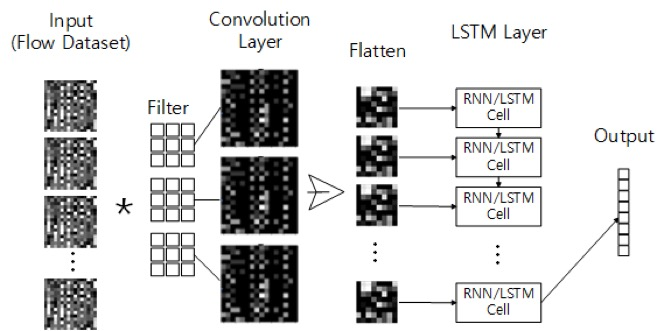
\includegraphics[width=3.6in]{fig6.jpg}
\caption{CNN and RNN combination learning model architecture}
\label{fig6}
}
\end{figure}